\noindent\textbf{Caso observado: sobreposição de percursos na linha 6L10-41}

Em 23 de outubro de 2026, durante os testes internos, os responsáveis pela implementação observaram que o percurso da linha 6L10-41, sentido Messiânica, parecia incorreto no mapa. O trecho contínuo posterior ao embarque encobria parte do tracejado anterior nos locais em que a linha passava novamente pela mesma via. Sem indicação do sentido, o desenho dificultava distinguir uma entrada no bairro seguida de retorno de uma ligação indevida entre ruas. A observação foi registrada no processo de desenvolvimento; não é atribuída a passageiro externo nem ao avaliador técnico.

A conferência da sequência de paradas do GTFS local e da relação de vias da SPTrans apresentada durante a análise identificou o percurso Terminal Varginha, Av. Jaceguava, Av. Prof. Hermann von Ihering, Rua Matilde de Lutis Barbosa, retorno pela Av. Prof. Hermann von Ihering, Av. Jaceguava e Av. do Paiol. Portanto, o retorno por parte das mesmas vias não constituía, isoladamente, evidência de erro de itinerário. A dificuldade de leitura motivou a inclusão de setas e de um pequeno deslocamento lateral dos traços conforme o sentido de circulação. Esse afastamento é apenas gráfico, em pixels: não altera as coordenadas cadastradas, as paradas ou o cálculo das viagens, e não representa a posição exata de uma faixa de trânsito.

\begin{figure}[H]\centering
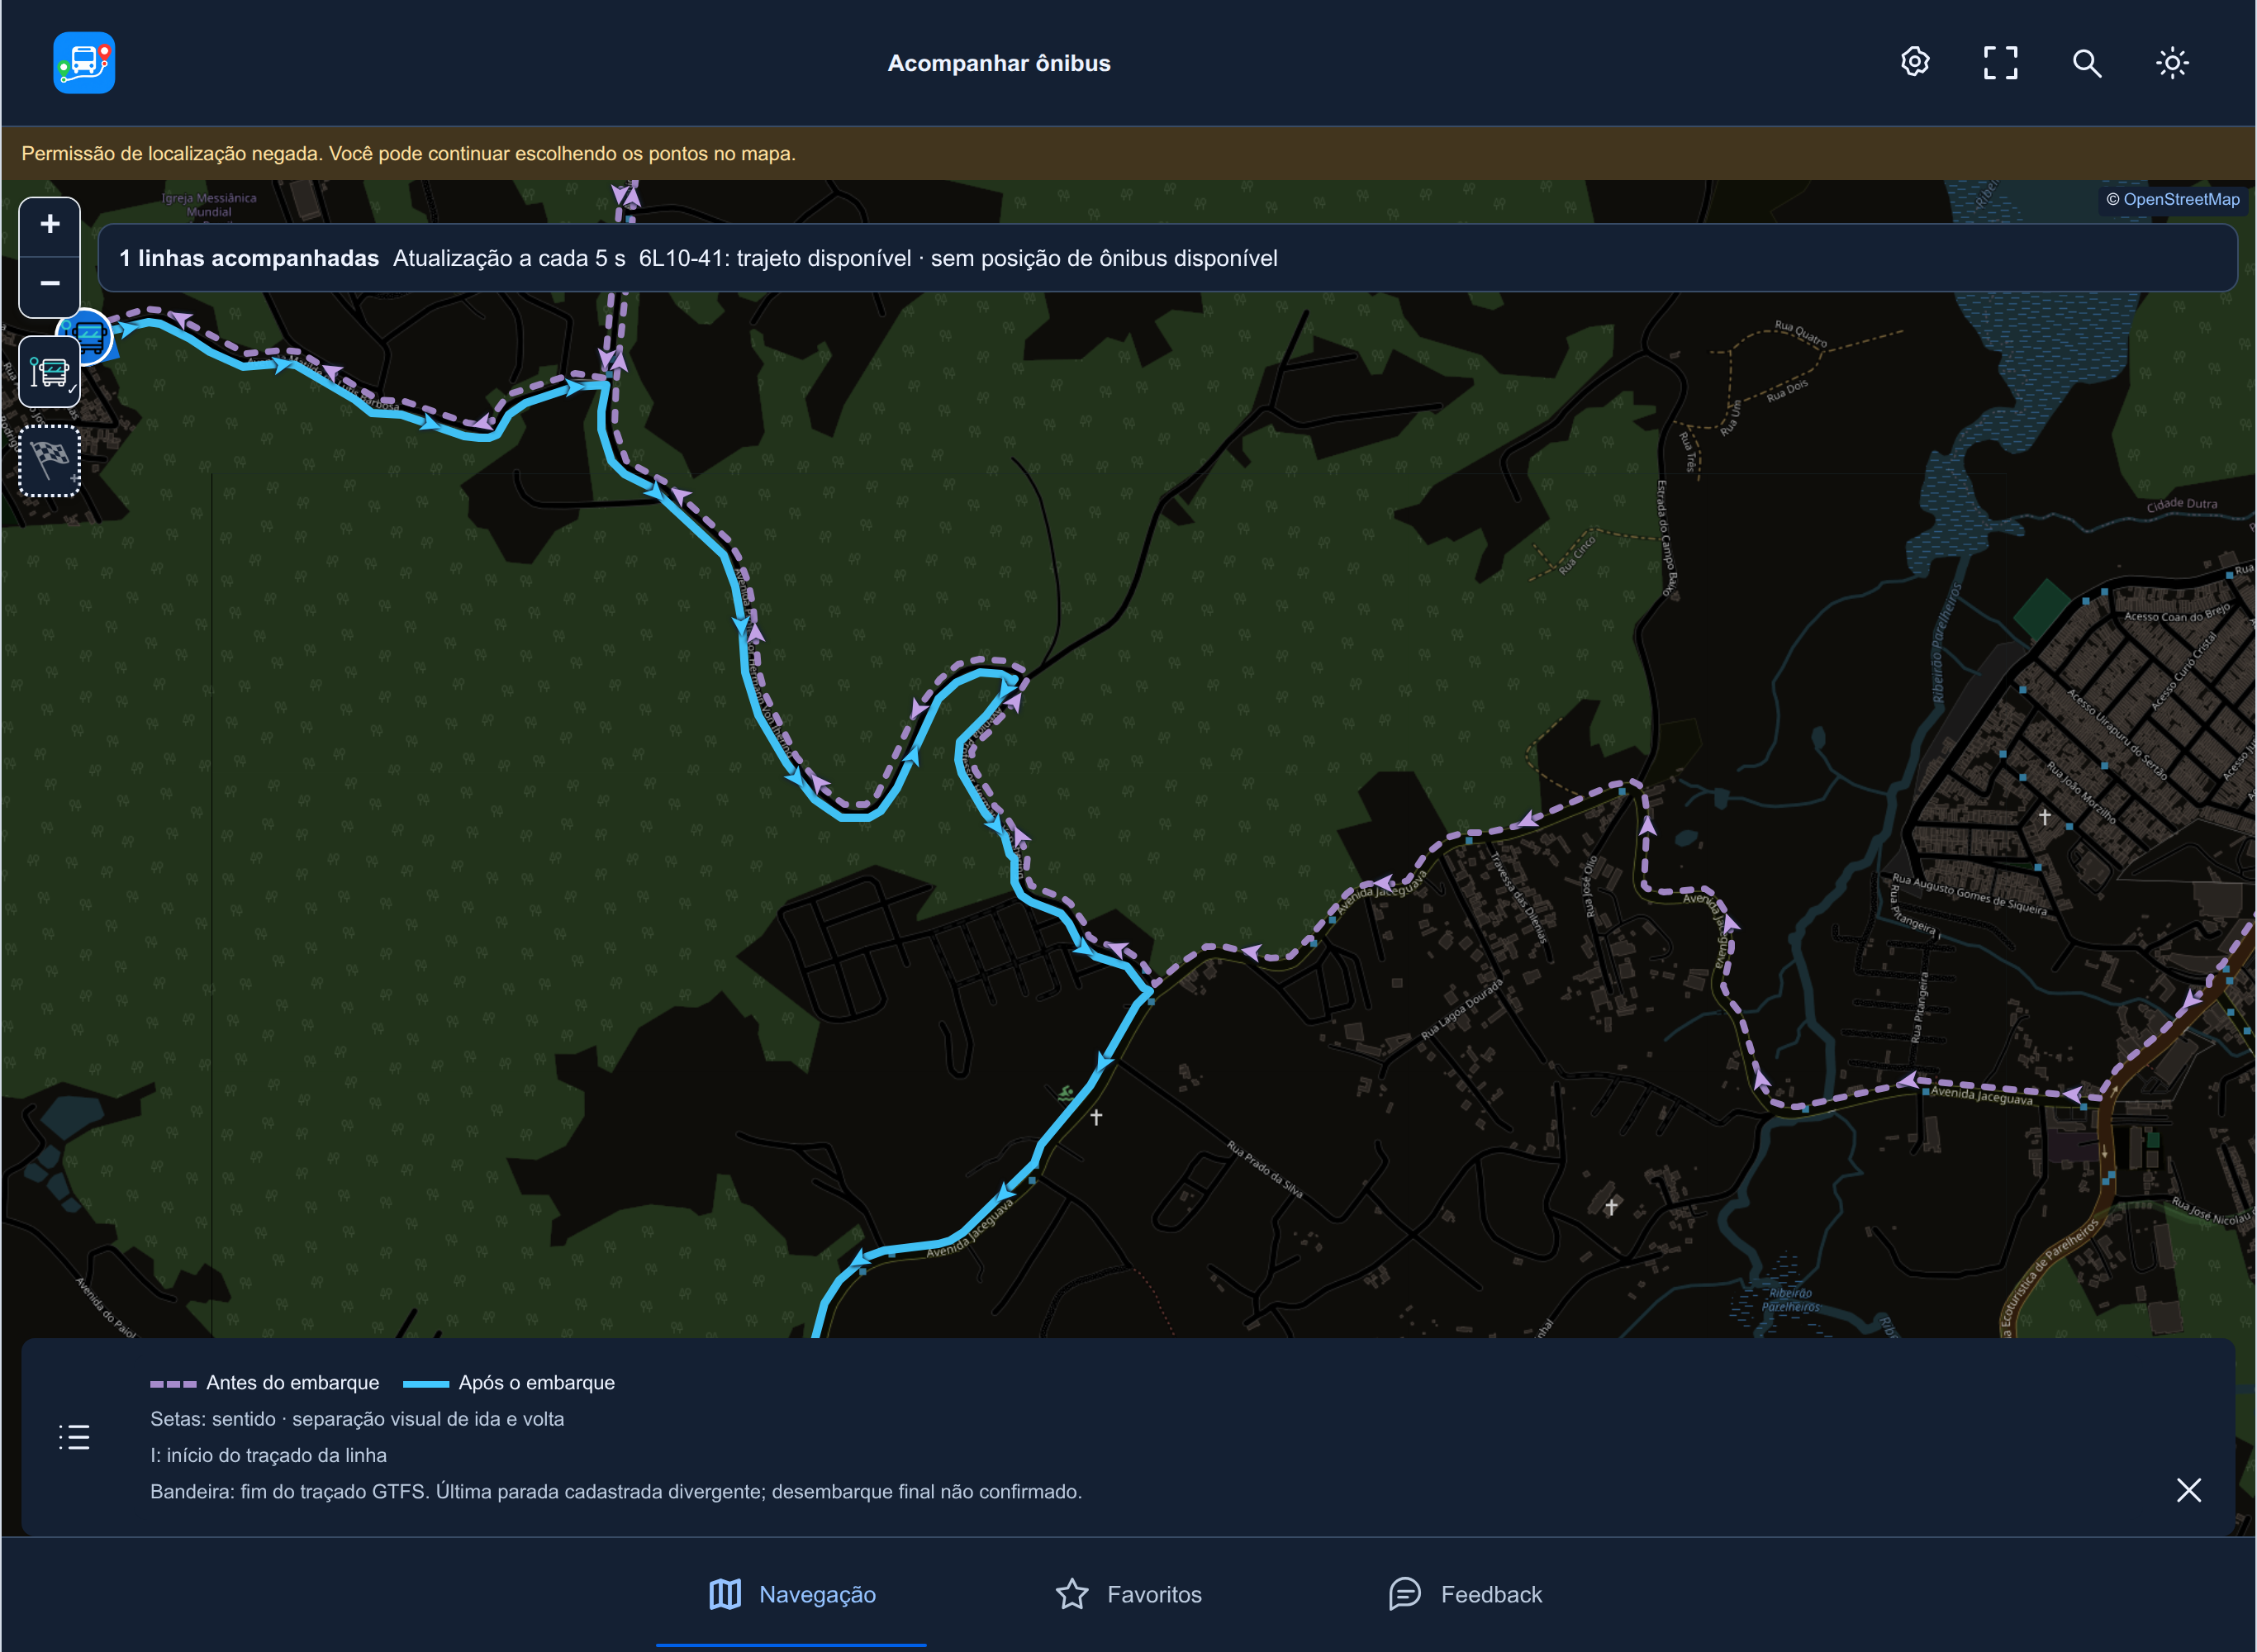
\includegraphics[width=\textwidth,height=0.56\textheight,keepaspectratio]{capturas/2026-10-23-rotas/linha-6L10-detalhe.png}
\caption{Detalhe da linha 6L10-41 após a correção: setas e separação visual das passagens em sentidos opostos.}\label{fig:rotas-sobrepostas}
\fonte{Captura real da aplicação, ampliada pelo controle de zoom do mapa, 23 out. 2026.}
\end{figure}

O lilás tracejado identifica a parte anterior ao embarque selecionado e o azul contínuo identifica a parte posterior. Esses estilos se referem ao ponto escolhido, não ao histórico de deslocamento de um veículo. O início é indicado por ``I'', e o botão de retorno à lista permanece à esquerda. A seleção do traçado completo também foi disponibilizada quando não há previsão ou posição de ônibus; ausência de informação operacional não impede consultar o itinerário cadastrado.

Foi identificada, separadamente, uma divergência entre a última parada cadastrada, Av. do Paiol, 1413, e o término da geometria da viagem \texttt{6L10-41-1}. Em vez de cortar o percurso ou criar uma parada não confirmada, a aplicação preserva o traçado e apresenta a bandeira como ``fim do traçado GTFS'', acompanhada da ressalva de que o desembarque final não está confirmado. Essa sinalização explicita a incerteza; não corrige nem valida operacionalmente a fonte de dados.

A verificação da mudança de direção visual incluiu testes automatizados com coordenadas artificiais, cobrindo percursos opostos e pontos repetidos, além de regressões em navegador para linhas com e sem veículos, acompanhamento individual e divergência do ponto final. Na execução registrada durante a implementação, passaram 49 testes unitários de frontend e quatro testes de navegador. Esses resultados verificam comportamento de software; não demonstram melhora mensurada de usabilidade. As capturas desta revisão utilizam dados reais e documentam o estado posterior à correção, sem reconstrução sintética de uma tela anterior.

